\section{Versuchsbeschreibung}

\subsection{Versuchsaufbau}
\begin{center}
	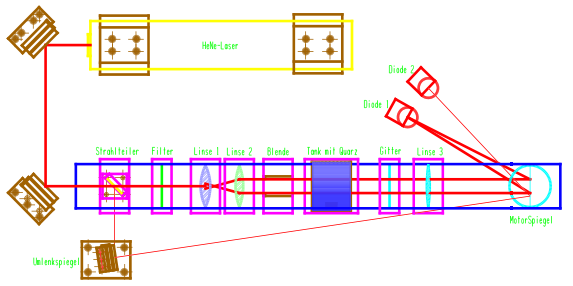
\includegraphics[width = \textwidth]{Bilder/Aufbau.jpg}
\end{center}


\subsection{Durchf\"uhrung}

Mit einem He-Ne Laser, der monochromatisches Licht der Wellenl\"nge $\lambda = 6328 \mathring{A}$ abstrahlt, untersuchen wir das Beugungsph\"anomen an verschiedenen Gittern und bestimmen daraus die Gitterkonstanten bzw. Aperturfunktionen dieser Gitter. Bei einem Ultraschallgitter versuchen wir au\ss erdem die Schallwellenl\"ange in einer Isooktan-L\"osung herauszufinden und vergleichen unsere Messergebnisse mit der Raman-Nath-Theorie.

\subsubsection{Sinusgitter}

Wir richten den Laserstrahl senkrecht auf das Sinusgitter ohne Aufweitung und ohne Kollimationslinse, da bei diesem Gitter die 0. und die 1. Ordnung problemlos unterscheidbar sind. Auf einem Schirm hinter dem Gitter kann man das Beugungsmuster direkt beobachten und somit die Gitterkonstante bestimmen.

\subsubsection{Amplitudengitter}
